% \section {Design} <cross>copy & paste</cross> well modify & revise it; justify the changes
\section{Design} \label{design}
\subsection{Anticipated components of the system}
\par\noindent
The main partition of the system was a software that enables to simulate
and visualise each interaction of a model before convergence (or termination, according to type of model) of this model. The project
would also attempt to explore one or more protocol to check their internal
status after finishing the software.

\par\noindent
The simulator would allow users to choose from a set of well-defined protocol and
specify the parameters for these protocol (e.g. number of agents participating).
The simulator would allow users to easily extend their own protocol though writing
structured few lines of Kotlin \cite{Kotlin} code.

\par\noindent
The system expected to have a ability to simulate some variations (which at
least includes the network constructor \cite{MS16a} and terminating grid network constructor in 2D \cite{Mi17})
of the original protocol according the protocol and dynamically visualise how process (nodes) transfer for each interaction.

\par\noindent
The software would be writing in Kotlin  \cite{Kotlin}. The interface provided would be a desktop application running on Java Virtual Machine Platform.
A web interface was desirable but would not be guaranteed to deliver.

\paragraph{Modification against original design} The original design mentioned it could include "a configuration parser to
  enable user define a protocol from configuration files" finally replaced by a set of
  well-defined set of protocol and a programmable interface. This is because the
  original design requires a design and implementation of Domain Specific Language (DSL),
  and a parser of this kind of "new language", which is a expected large work load and might be
  infeasible to finish all of them
  during the project period. This might be included in the following development plan
  after finishing the project.

\subsection{Data structure, algorithms and pseudo-code for key method}
\subsubsection{Graph and adjacency list}
\par\noindent
For some specific kinds of model, specifically ,the network constructor, a data
structure to maintain an undirected graph $G$ given by current configuration $C$ is required. In other words, it requires to maintain
a group of status of $active$ edges. It aims to construct ”shapes”
and there are some status for the edge $uv$ in between any nodes (processors) $u$
and $v$ in the population.

\par\noindent
To achieve this, an adjacency list would be used to record the connections associated
with each nodes. Initially, it would be an map with all nodes in the population
as keys and an empty list associated as the value. If the connection in between $u$ and $v$ builds up,
the node $u$ will be added to the list which the node $v$ corresponds to and vice versa
(i.e. the $v$ will be added to the list which the key $u$ corresponds to). When an $active$
connection, say a connection between $u^{'}$ and $v^{'}$ "cancelled" (i.e.
running from $active$ state to $inactive$ state), the node reference $v^{'}$ in the list that
$u^{'}$ as the key would be deleted and so the node reference $u^{'}$ in the list that
$v^{'}$ as the key.

\paragraph{Modification against original design}
The original design used an adjacency matrix rather than a adjacency list to represent the
undirected graph that possibly appeared in some model to be simulated. The modification was made based on
the consideration on space cost. A adjacency matrix requires a fixed $S(N^{2})$ space allocated overhead
for $N$ nodes in the population while the proposed adjacency list implementation would consume $S(E)$ where
$E$ is the number of $"active"$ edges, which at most has a value of $\frac{N * (N - 1)}{2}$.


\par\noindent
For every model defined, the initial configuration always starts with no $active$ edge so it would be a zero matrix if
the adjacency matrix is used in the program and would need to maintain a sparse state for most of time during simulation process.
A adjacency list might be a better choice since the list would save spaces required than adjacency matrix.

\subsubsection{Quad-direction linked structure}
In 2-dimensional case, the agents in grid terminating grid network constructor model would have exactly 4 ports associated with them and
any edges have to be connected through ports. As mentioned before, the port themselves are perpendicular with each other.
To implement port concept and connection attached to ports,
the system would use a quad-direction linked structure to construct this. Each nodes would have 4 null-able references to other
nodes, one of which represents a port associated to this node. A connection (or edge) $e$ between node $n$ and node $n^{'}$ is treaded as "active" on a port $p$ of $n$ if the reference that
$p$ associated pointing to an another non-null node $n^{'}$ and so similar for the symmetric reference in $n^{'}$.
In contrast, the connection (or "edge") on a port is deemed as "inactive" if the port reference pointing to null.

\par\noindent
\begin{lstlisting}[caption = {Pseudo-code demonstration of quad-direction linked structure}, style = mykotlin]
  class LocallyCoordinatedModelNode(...){
    var up: LocallyCoordinatedModelNode? = null
    var down: LocallyCoordinatedModelNode? = null
    var left: LocallyCoordinatedModelNode? = null
    var right: LocallyCoordinatedModelNode? = null
    ...
  }
\end{lstlisting}

\paragraph{Relative node coordinate and rotation}
For convenience of implementation, the relative node coordinate would be defined here. Given
a node $n$, with it coordinate $(x_{n}, y_{n})$. The nodes that connected to its port $p_{x}, p_{-x}, p_{y}, p_{-y}$
will have coordinate $(x_{n} + 1, y_{n}), (x_{n} - 1, y_{n}), (x_{n}, y_{n} + 1), (x_{n}, y_{n} - 1)$ respectively.
Note that the coordinate is localized and from different node, they will have a different perspective of coordinate.
It is also required to define a parameter $\varphi_{i}$ representing the rotated degree from normal Cartesian coordination.
Here, the "positive" direction can be defined as clockwise.

\paragraph{Relative port degree}
In terminating grid network construction model, the 4 ports associated a node is called
port $p_{y}$, $p_{x}$, $p_{-y}$ and $p_{-x}$, may simply donated as $u$(UP), $r$(RIGHT), $d$(DOWN) and $l$(LEFT), respectively.
They are perpendicular to each other. To model the perpendicularity of node numerically,
it proposed to notate a degree for each port. Specifically, $u$(UP) is with a degree value of
\ang{0},  $r$(RIGHT) is with a degree value of \ang{90}, $d$(DOWN) is with a degree value of
\ang{180} and $d$ is with a degree value of \ang{270}.

\par\noindent
\begin{figure}[H]
\begin{center}
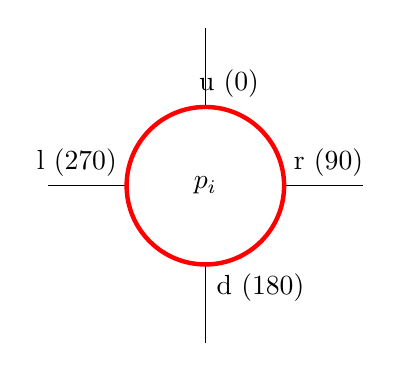
\begin{tikzpicture}
    \draw (2,0) -- (2,1);
    \draw (2,4) -- (2,3);
    \draw (0,2) -- (1,2);
    \draw (4,2) -- (3,2);
    \draw [red, ultra thick] (2,2) circle [radius=1];
    \node [below] at (2.7,1) {d (\ang{180})};
    \node [above] at (2.3,3) {u (\ang{0})};
    \node [left] at (1,2.3) {l (\ang{270})};
    \node [right] at (3,2.3) {r (\ang{90})};
    \node [label] at (2,2) {$p_{i}$};
\end{tikzpicture}
\end{center}

\caption{Defined degree for each port}
\label{standardR}
\end{figure}

\par\noindent
The difference $\theta$ of degree between two ports $p_{1}$, $p_{2}$ can be defined as
$$ \theta = ||\theta_{1} - \theta_{2}|| = ||Angle(p_{1}) - Angle(p_{2})||$$
where $Angle$ is a mapping from a port $p_{i} \in \{ p_{y}, p_{x}, p_{-y}, p_{-x}\}$
to its degree $\theta_{i} \in \{\ang{0},\ang{90},\ang{180},\ang{270}\}$.
Suppose there two nodes $a$, $b$ and two ports where $p_{a}$ is
one port of $a$ and $p_{b}$ is one port of $b$, then the \textbf{"relative difference"} $\Theta$ could be:
\begin{equation} \label{Equ_port_differ}
\Theta_{p_{ab}} \equiv ||\theta_{p_{a}} - \varphi_{a} - (\theta_{p_{b}} - \varphi_{b})|| \bmod 360
\end{equation}
which is the port difference after involving the rotation of nodes.

\paragraph{Relative docking port \label{dockerport}}
Also for convenience of implementation, here two pairs of "relative docking port" would
be defined. A pair of relative docking port is the pair of ports of which relative
difference is \ang{180}. Certainly, if the rotation of nodes is not involved, this limits only two possible pairs of
relative docking port: port $\{p_{x}, p_{-x}\}$ as the first pair of docking port,
and port $\{p_{y}, p_{-y}\}$ as the second pair of docking port. Suppose there are
two nodes shown as exactly in diagram \ref{standardR}, that is, two nodes with \ang{0}
rotations and if assuming there is no rotation allowed in the configuration, the only legal connection will
be connections in between the two pairs of relative docking port,
where the two ports belonging to different nodes and the two nodes can be interchangeable.
For instance, suppose the port of the first node is selected as $p_{x}$, then the only legal
choice for the port of the second node is $p_{-x}$, which is the relative docking port of $p_{x}$.


\paragraph{Breadth-First Search (BFS) Algorithm \cite{Cormen:2009:IAT:1614191} on Quad-direction linked structure}
Breadth-First Search (BFS) algorithm is a famous and broadly-used graph traversing algorithm and is also
foundation for some other algorithm \cite{Cormen:2009:IAT:1614191}. Here, it would not be repeated for the
details of BFS algorithm but there is a modification when applying the algorithm the Quad-direction linked structure.
Because there are four nodes reference (edge) attached to one node, it treat all the 4 references as possible source of "son nodes" and if
any of them are not null and also had not been visited, they will be marked and be added to the tail of a queue for further traversal.

\par\noindent
Consider a \textit{clique} or a connected (sub - )graph in a configuration for the terminating grid network constructor model,
the BFS can be used to aggregate this kind of clique from any node inside that clique as a set. This set of nodes can be used
as an input for a function applying on a batch of nodes in a same clique, for instance, rotating all nodes according to a centred node.

\subsubsection{Terminating grid network constructor: Check acceptable configuration \& Handle rotation}
\paragraph{Problem: Detecting legal configuration}
As mentioned in background section, not all possible configurations are acceptable, or say, belong to $A(C)$ given the geometrical restriction\cite{Mi17}.
Hence, this will requires some inspections to ensure that only the acceptable configurations appears
after a node interacts with each other during simulation process. There are two ways to finish this kind of inspections:
\begin{enumerate}
  \item List all possible interactions at each discrete step, filter out
  all illegal ones to get $A(C)$, and then select one configuration from $A(C)$.
  \item Select one possible interaction from all possible interactions, reject if the interaction forms a configuration $c_{w} \not\in A(C)$
  and repeat the process until a acceptable configuration is found. The entire process would be happened in one discrete step.
\end{enumerate}
The second approach is more feasible since it supposed to cost a impracticable long time to enumerate all possible elements in $A(C)$ at a particular discrete step.
Hence, it would be discussed for what kind of cases should be rejected for an interaction.

\paragraph{Avoid self-connection}\noindent
Recall the definition of transition function of grid network constructor, two nodes and two edges associated with the two nodes respectively are selected.
This not excludes the case that one same node identity is selected twice, which leading to a
unsound connection on the selected node itself. This could be avoided through prohibiting the second selection to select an entity as same as the first selection.
\begin{figure}[H]
\begin{center}
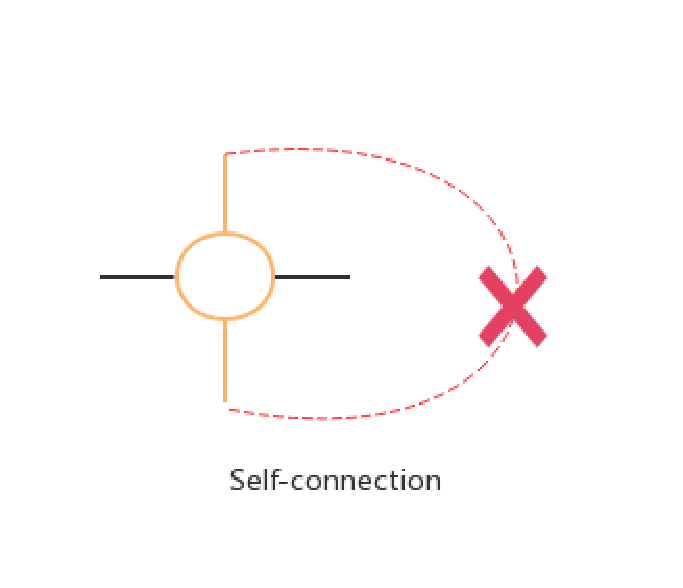
\includegraphics[width = 0.5\textwidth]{context/diagram/self-connection.pdf}
\caption{Illegal configuration: Self-connection}
\label{selfcon}
\end{center}
\end{figure}

\par\noindent
\paragraph{Avoid unit-distance violation}\noindent
A connection in models of terminating grid network constructor has to follow the unit distance restriction.
\begin{figure}[H]
\begin{center}
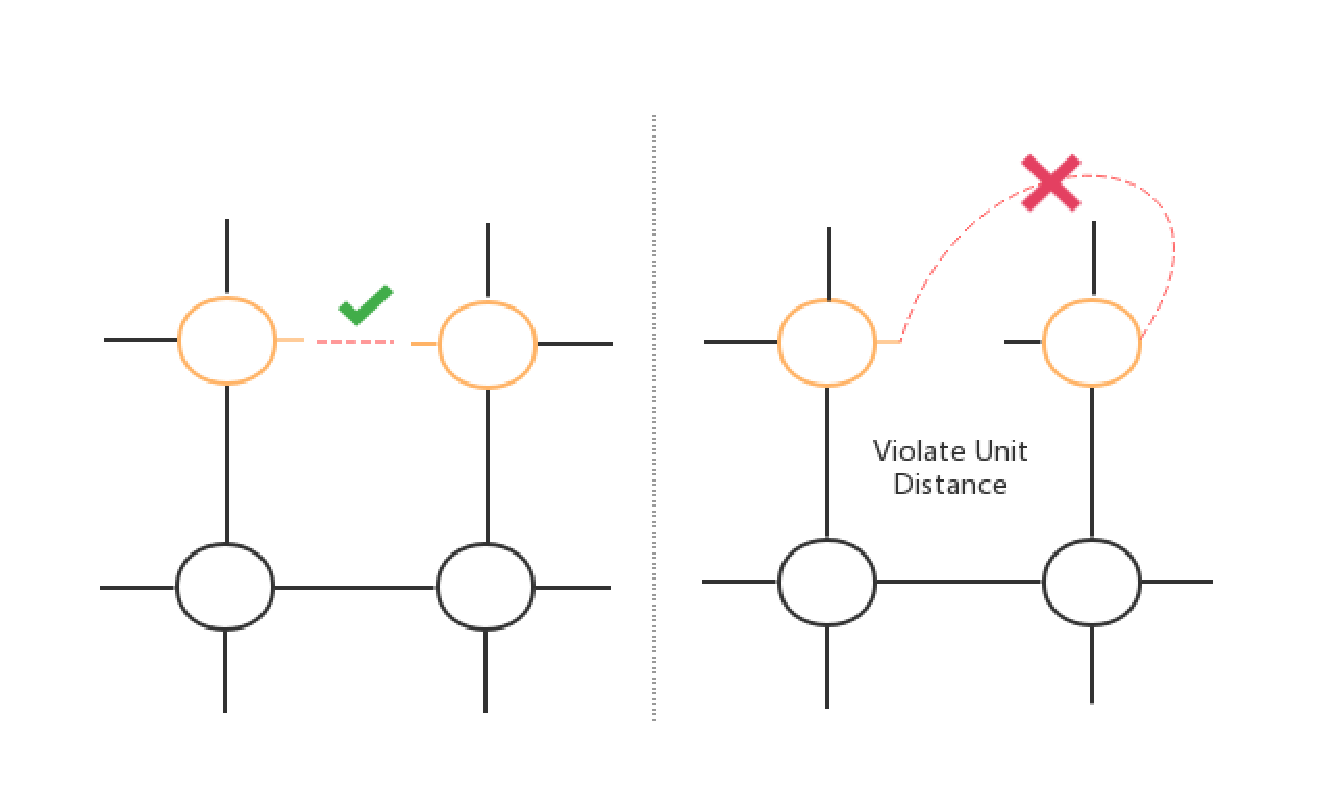
\includegraphics[width = 0.8\textwidth]{context/diagram/unitDistanceViolation.pdf}
\caption{Illegal configuration: Unit distance violation}
\label{unitvio}
\end{center}
\end{figure}
\par\noindent
As illustrated in diagram \ref{unitvio}, the left-hand side configuration is acceptable but the right-hand side configuration is not because
it violates the unit distance. After the connection in the right-hand side being active, the configuration will not be sub-graph of 2-D grid network
with unit distance restrictions.

\par\noindent
It can be noticed that unit distance violation always happens when two interacting nodes are belonging to one
same clique since a rotation will helps if the two nodes are in different cliques. The condition
that two nodes are in the same clique simplifies the judgement process. First, it requires to check the
whether the selected two port are docking port according to equation \ref{Equ_port_differ} (so this ensures after activating connection the
direction of two ports will conform the grid network restriction). If the two ports selected are a pair of
docking port, the initializer node then will mark itself with coordinate $(0,0)$ and populate the coordinate using
BFS algorithm. Finally, it will check the Euclidean distance of the two interacting nodes using propagated coordinates,
which is asserted to be 1 otherwise it means that unit-distance restriction will be broken after interaction.

\begin{algorithm}
\caption{Algorithm for detecting unit distance violation}\label{algo_dudv}
\begin{algorithmic}[1]
\Procedure{Detect}{}

\State $((\textit{nodeA},\textit{portA}), (\textit{nodeA}, \textit{portA}) \gets \textit{scheduler.select()}$
\State $\textit{isViolation} \gets false$
\If {$\textit{nodeA.belongToGroup} \not= \textit{nodeB.belongToGroup}$} \Return \textit{isViolation} \EndIf
\If {$\textit{isDockingPort(portA, portB)}$}
    \State $ nodeA.coordinate \gets (0,0) $
    \State $ connectedSet \gets bfsForPopulatingCoordinate(nodeA) $
    \State $ distance \gets euclideanDistance(nodeA \in connectedSet, nodeB \in connectedSet)$
    \If { $distance \not= 1$} \State $\textit{isViolation} \gets true$ \EndIf
\Else
    \State $\textit{isViolation} \gets true$
\EndIf

\Return \textit{isViolation}

\EndProcedure
\end{algorithmic}
\end{algorithm}


\paragraph{Avoid overlapping}\noindent
Overlapping is another situation that persuades a configuration become an acceptable
configuration. This normally happens when two nodes that belongs to different cliques
interacting with each other. This is not allowed for some cases when more than one nodes
appears in the same position.
\begin{figure}[H]
\begin{center}
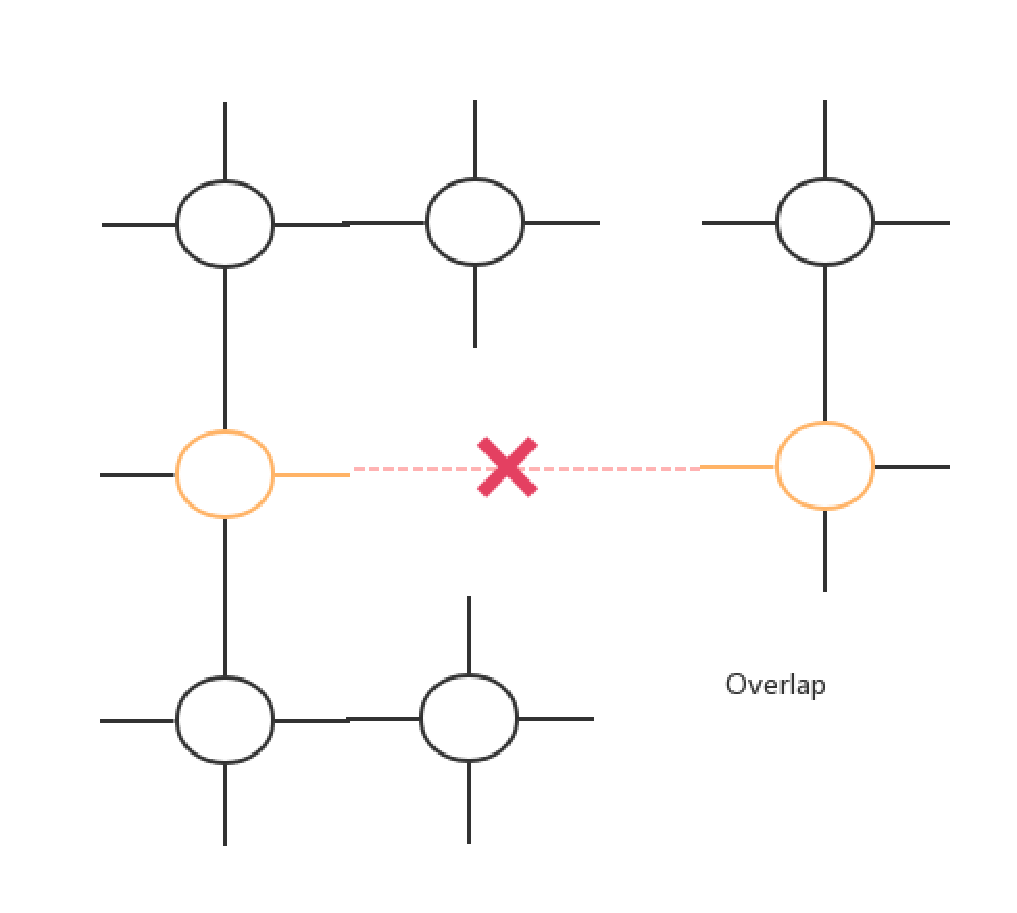
\includegraphics[width = 0.5\textwidth]{context/diagram/overlap.pdf}
\caption{Illegal configuration: Unit distance violation}
\label{overlap}
\end{center}
\end{figure}
\par\noindent
The figure \ref{overlap} presents an interaction for highlighted nodes and edges.
This kind of interaction should be rejected because it causes an overlap. To check on this, it can be assumed that
the interaction had already done and see whether there is at least one pair of nodes
owning a same coordinate. If it does, the interaction should be rejected because it causes
an overlap otherwise it should accept the interaction.

\par\noindent
Note that after populating the coordinate, the coordinates of nodes in clique that the receiver belonging to
is based on the receiver nodes' perspective. Hence, these coordinates of nodes require to do a centralized rotation with receiver as the center to
confirm to the coordinates from initializer's perspective. The rotation degree is given by
$$180 - ||Angle(port_{receiver}) - Angle(port_{initializer}))||$$ which is the "port difference without node rotation involves", because the internal
shape of two cliques is no related to their rotation degree).

\par\noindent
Some cases might be more complicated. The two cliques may overlap with each other but their axisymmetric one will not. An example could be:
\begin{figure}[H]
\begin{center}
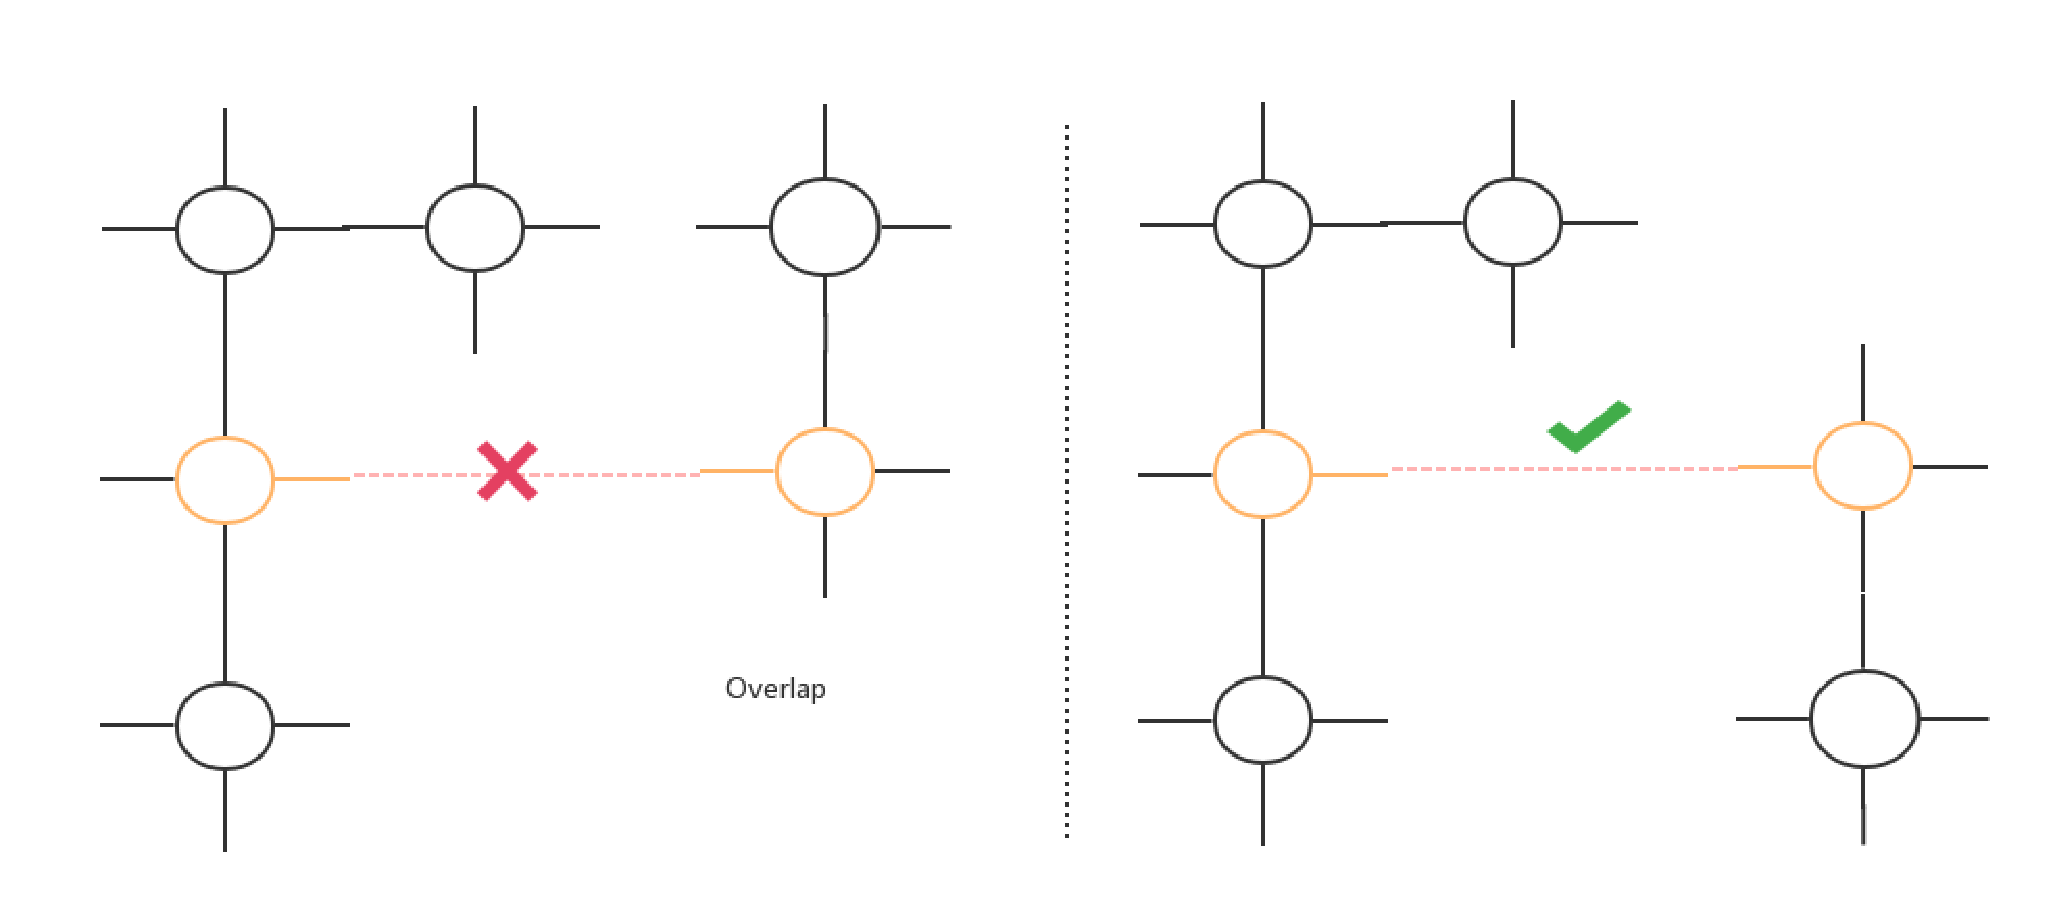
\includegraphics[width = 0.5\textwidth]{context/diagram/overlap_flipping.pdf}
\caption{Axisymmetric shape eliminate overlap}
\label{overlap_flipping}
\end{center}
\end{figure}
\par\noindent
The two cliques will be overlapped with each other after interaction in the left-hand of the figure \ref{overlap_flipping} but if one of them
flip about the "x-axis" of another clique the overlap will be eliminated. For interaction happens with $p_{x}$(RIGHT) and $p_{-x}$(LEFT) of initializer node, it may need to check the
clique that the receiver node belongs to and its x-axisymmetric shape. For interaction happens with $p_{y}$(UP) and $p_{-y}$(DOWN) of initializer node, it may need to check the
clique that the receiver node belongs to and its y-axisymmetric shape.

\begin{algorithm}
\caption{Algorithm for detecting overlapping}\label{algo_do}
\begin{algorithmic}[1]
\Procedure{Detect}{}

\State $((\textit{nodeA},\textit{portA}), (\textit{nodeA}, \textit{portA}) \gets \textit{scheduler.select()}$
\State $\textit{isOverlap} \gets false$
\If {$\textit{nodeA.belongToGroup} = \textit{nodeB.belongToGroup}$} \Return \textit{isOverlap}
\Else
    \State $ nodeA.coordinate \gets (0,0) $
    \State $ connectedSetA \gets bfsForPopulatingCoordinate(nodeA) $
    \State $ nodeB.coordinate \gets getCoordinateReceiver(nodeA, portA)$
    \State $ connectedSetB \gets bfsForPopulatingCoordinate(nodeB) $
    \State $ connectedSetB \gets bfsForRotation(connectedSetB, 180 - ||portB.angle - portA.angle||) $
    \State $ symmetricSetB \gets symmetric(connectedSetB, portA)$
    \If { $(connectedSetA$ $\cap$ $connectedSetB \not= \emptyset)$ $\land$ $(connectedSetA$ $\cap$ $symmetricSetB \not= \emptyset)$}
      \State $\textit{isOverlap} \gets true$
    \Else
        \If {$(connectedSetA$ $\cap$ $connectedSetB \not= \emptyset)$}
          \State $changeToSymmtricStructure(nodeB, portA)$
        \EndIf
    \EndIf
\EndIf

\Return \textit{isOverlap}

\EndProcedure
\end{algorithmic}
\end{algorithm}


\paragraph{Modification against original design}
This section is the solution towards the legal configuration checking problem in
original design document. The original version proposed such a problem without answers.
For now, the solution have been figured out.

\subsection{Interaction (Sequence) Design}
\begin{figure}[H]
\begin{center}
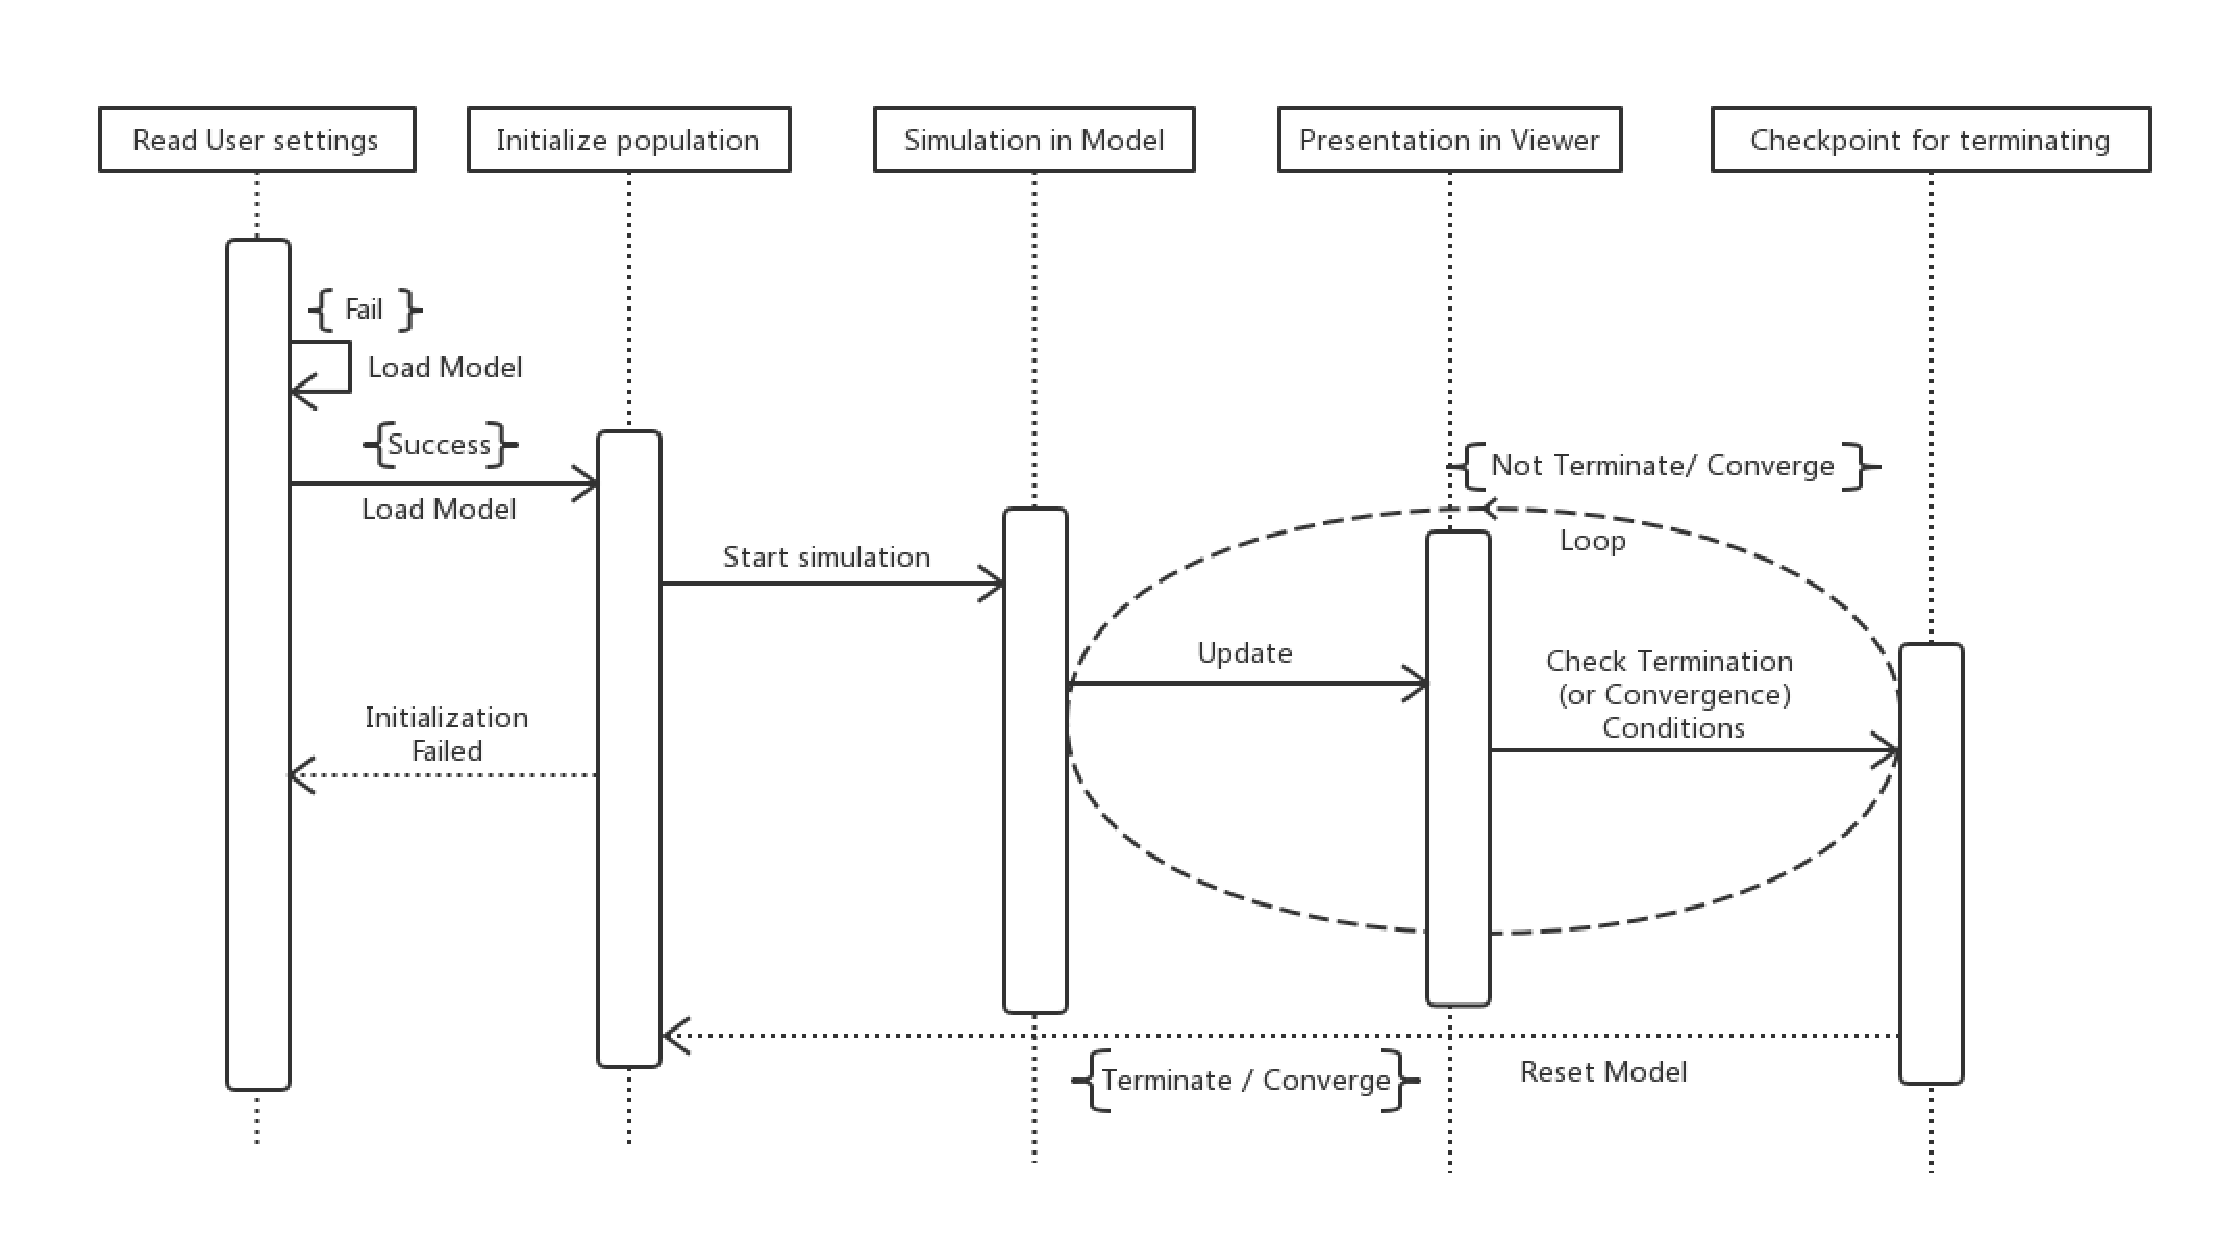
\includegraphics[width =\textwidth]{context/diagram/interaction.pdf}
\caption{Interaction Design Diagram}
\label{interactionG}
\end{center}
\end{figure}

\par\noindent
The figure \ref{interactionG} illustrates the entire interaction process of the
simulator. Initially, the users select one protocol from a set of well-defined
protocols and then select or input a set of parameters such as how many nodes to
be included in the simulation, the initial status distribution for nodes and so forth.
Then the user click the "Apply settings button" to apply the model settings. Before
applying the model, the program itself would check whether all parameters are
well-defined, i.e. locating in the value range they should be. If they are, the software
would load the model otherwise it will reject this particular request from user and
allow the users to attempt their (possibly) another setting.

\par\noindent
After the program successfully loaded a model, the user can press the "Start simulation"
button to start a simulation. A simulation contains multiple steps. For each step,
the model executes interactions under the control of scheduler specified in one
of parameters mentioned before and then the model would update the states of elements
 in viewer to show the what happened in the model itself. Following that, the model would
 check whether it reaches a configuration that should stop the simulation. A stop can be caused
 by user's temporarily interruption (pause) or the fact that the number of consistent accumulation of
 inefficient interactions overwhelms a pre-configured parameters defined in the model (which indicates
 a termination or convergence with a high possibility). If the model does not detect a stop,
 it will continue the "interact - update - checking stop" process in each step as a loop. Once it detects a
 stop, the software will return to the state that waits for starting of another simulation process
 (while the model would keep its internal states and user can build an another new model using a different set of parameters under this situation).

 \paragraph{Modification against original design}
The current design removed a step of sequence in original sequence design called "Initialize scheduler", which located after "Initialize population" state.
the "Initialize scheduler" process had been integrated into "Initialize population" because
the scheduler partition does not necessarily separated from the population and can be treated as a partition of a "population" in concept.

\subsection{UI Interface Design}
\begin{figure}[H]
\begin{center}
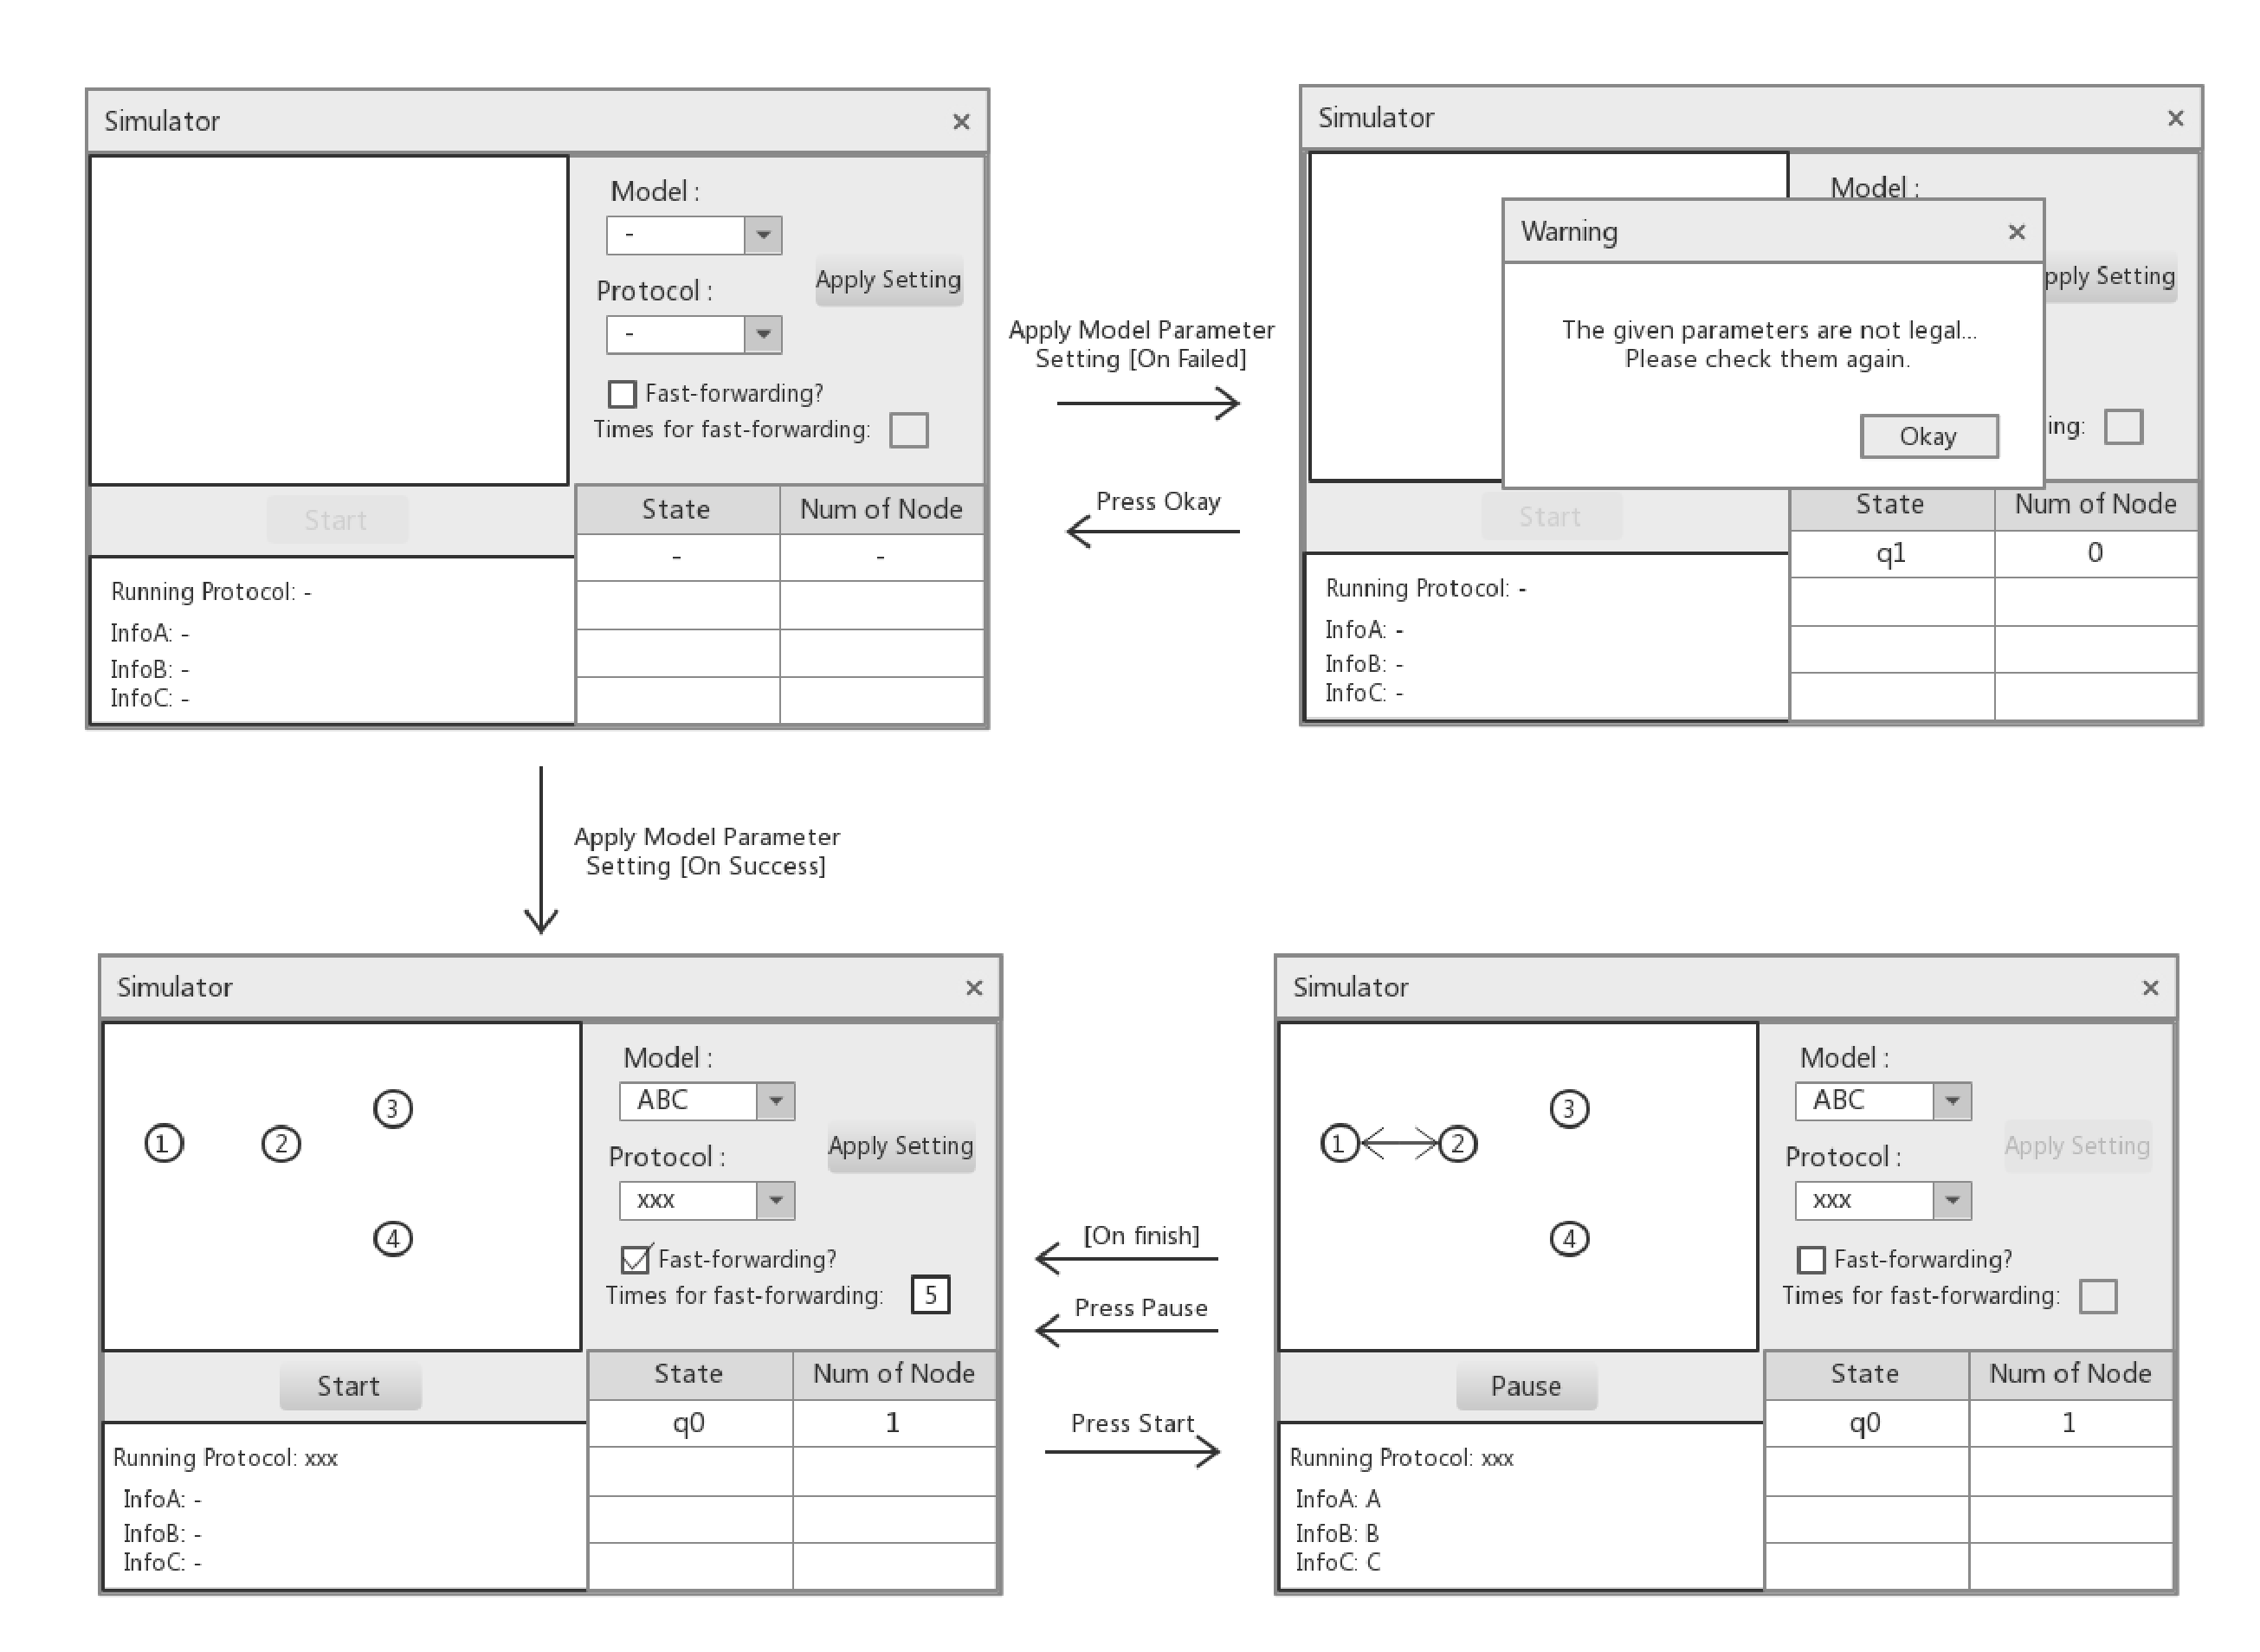
\includegraphics[width =\textwidth]{context/diagram/interface.pdf}
\caption{Interaction Design Diagram}
\label{intefaceG}
\end{center}
\end{figure}

\paragraph{Modification against original design}
The UI was redesigned entirely. This is because the original design built on the assumption
that the users load their settings for some population from domain specification language (DSL) codes residing in
some files. The DSL is infeasible to be finished due to the limited time of implementation.
Hence, the design would allow user to set their population through the UI containing a set of well-defined
protocols and would allow the users to write their own extensional protocol through few lines of codes.
As the functionality changes, the UI removed the functionality entrance for "loading files from disk" and
added some options to allow user setting the parameters of a protocol.

\subsection{Object used in the system}
\FloatBarrier
\begin{figure}[H]
\begin{center}
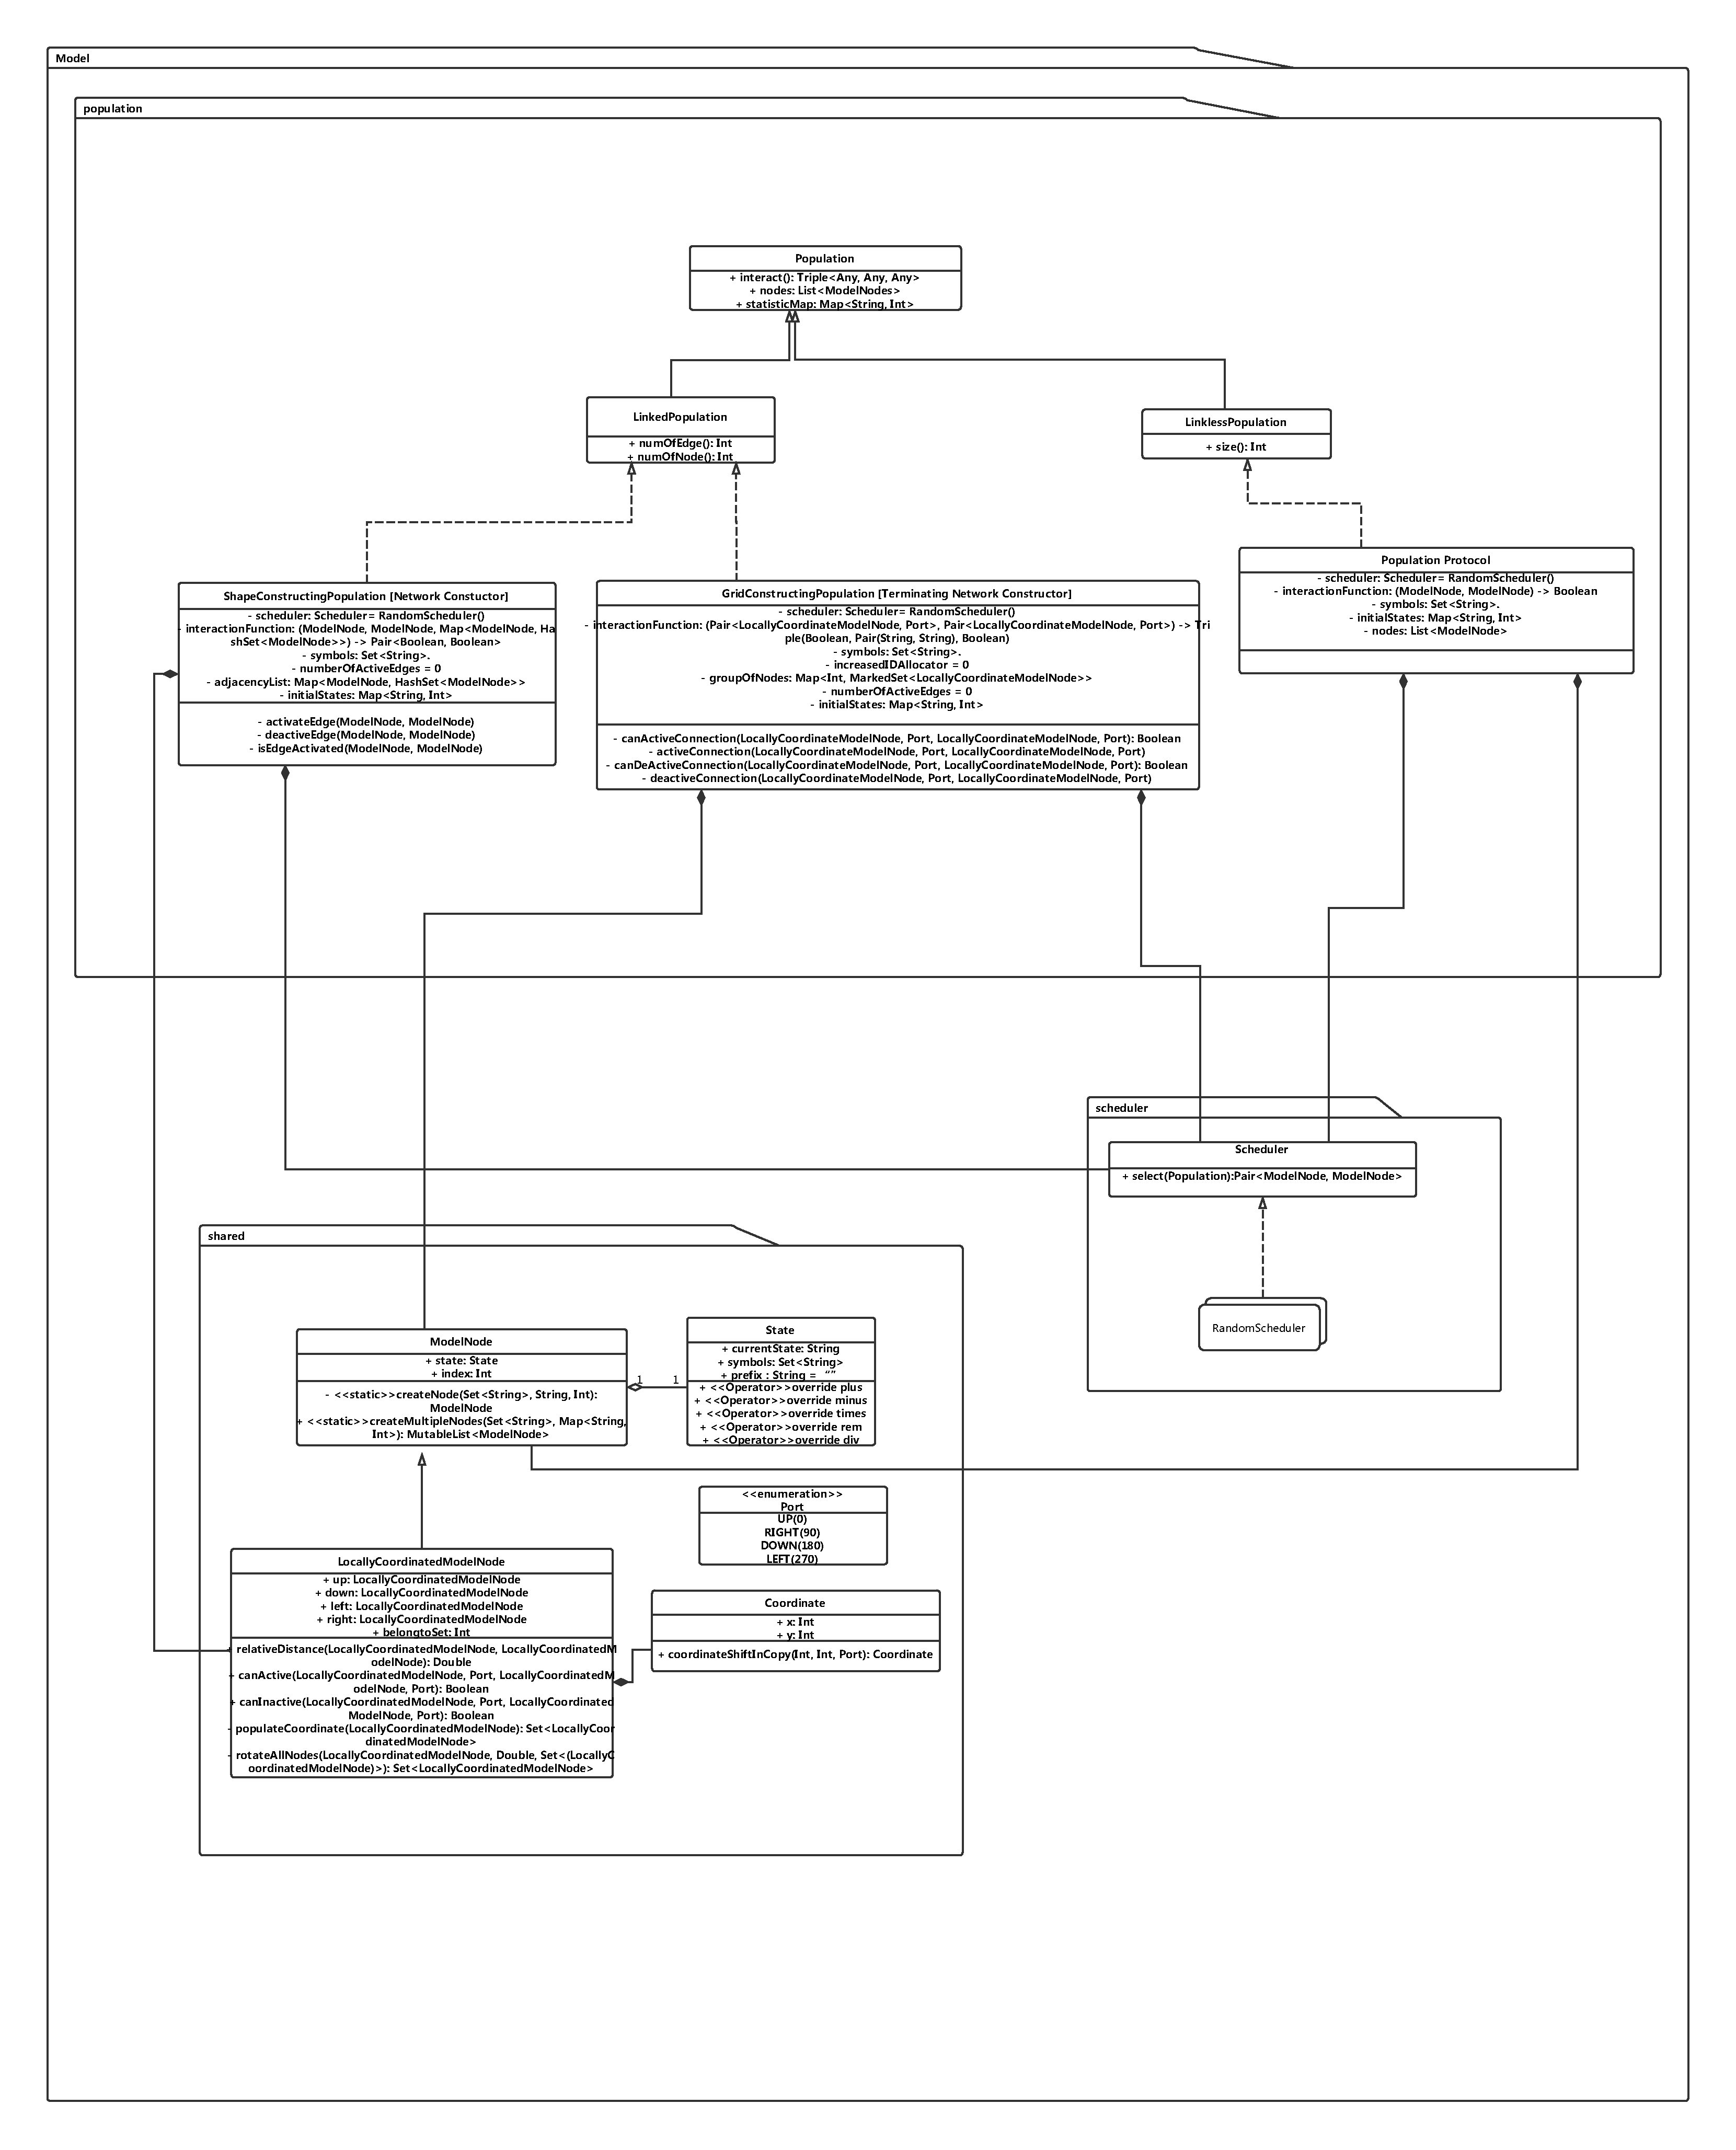
\includegraphics[width =0.95\textwidth]{context/diagram/uml_model.pdf}
\caption{Object-oriented Design: Model Part}
\label{oomG}
\end{center}
\end{figure}
